 
   %judul bisa diketik ulang
  \setstretch{1}%\small
  \begin{center}
      \textbf{\large \Title}\\
      \bigskip 
  \end{center}
  
  
  
  %Nama authors
   \begin{center}
     \bf \Author$^1$, Parman Sukarno$^2$, Erwid M. Jadied$^3$ 
  \end{center}
  
  
  %Afiliasi dan email
   \begin{center}
     $^{1,2,3}$Fakultas Informatika, Universitas Telkom, Bandung\\
%$^4$Divisi Digital Service PT Telekomunikasi Indonesia\\
$^1$hasobiroid@student.telkomuniversity.ac.id, $^2$psukarno@telkomuniversity.ac.id,\\ $^3$jadied@telkomuniversity.ac.id %$^4$pembimbingluar@telkom.co.id 
  \end{center}
  
   
 %%% Abstrak Indonesia %%%%%%%%%%  
   
{\bf \parindent0pt \noindent\rule{\textwidth}{1pt}
Abstrak

Perkembangan internet membawa dampak besar bagi kehidupan manusia, tetapi tidak semua hal yang berawal dari internet adalah efek yang positif, ada juga yang engatif. Salah satunya adalah ancaman kejahatan yang bertambah melalui internet atau cybercrime. Salah satu bentuk cybercrime adalah DoS, DoS adalah serangan pada jaringan yang sederhana namun efektif, beberapa kerugian besar telah diakibatkan oleh DoS. Dengan adanya permasalahan diatas maka kebutuhan akan pendeteksian DoS semakin penting, pada penelitian ini diusulkan sistem pengklasifikasian DoS dengan keakurasian deteksi diatas 80\% \cite{ddosfuzzy}\cite{ddosfpga}\cite{ddosrbf}. Penyerdahaan pada label juga menjadikan waktu \textit{training} lebih cepat dan akurasi tetap terjaga.

 \bigskip
Kata kunci : DoS, klasifikasi



%%% Abstrak English %%%%%%%%%%  

\noindent\rule{\textwidth}{1pt}
Abstract

The development of internet brings tremendous effect to human's life, but not all of it are positive effect, there are also negative effects. Cybercrime is one of it's result. One of cybercrime is DoS, DoS is a simple attack to internet network but quite effective, some losses were caused by DoS. Therefore a system to detect DoS is needed urgently, in this research will be proposed a sistem to classify DoS with accuracy more than 80\% \cite{ddosfuzzy}\cite{ddosfpga}\cite{ddosrbf}. There's also simplified labels which caused training time decreased but accuracy keep in the same level.

 \bigskip
Keywords: DoS, classify

\noindent\rule{\textwidth}{1pt} }



%%%%%% isi paper %%%%

\section{Pendahuluan}

\noindent\textbf{Latar Belakang}

Perkembangan internet dapat dikatakan pesat semenjak pertama kali digunakan untuk kepentingan militer dan akademik di Amerika Serikat, kini internet sudah mencakup segala aspek kehidupan manusia, mulai dari bidang komunikasi, Pendidikan, hiburan, hingga perbankan. Kompleksitas teknologi yang ada didalamnya pun semakin berkembang dari masa ke masa. Selain itu, ancaman kejahatan siber juga sudah muncul dari tahun 1820 meski saat itu belum ada internet. Kejahatan siber modern ini menyasar kepada data-data pribadi seperti alamat email, data kartu kredit, alamat rumah, detil identitas d.l.l.

Salah satu jenis serangan internet adalah DoS, serangan DoS pertama kali yang terdokumentasikan adalah pada 7 Februari 2000 yang menimpa beberapa situ e-commerce di Amerika Serikat seperti Amazon, e-Bay. Sejak saat itu serangan DoS terus berkembang dan berevolusi menjadi lebih efektif  dan berbahaya. Contoh serangan DoS lain yang menarik perhatian dunia adalah serangan DoS di Estonia pada tahun 2007, dimana serangan DoS di negara itu dapat melumpuhkan jaringan internet seluruh negara \cite{politicsofddos}.

Dari kejadian-kejadian diatas, dapat dilihat bahwa DoS memiliki peran dan tingkat berbahaya yang tinggi, hal ini mendorong peneliti-peneliti di dunia untuk mempelajari DoS dan melakukan deteksi lebih awal terhadap serangan DoS. Deteksi serangan dengan DoS dapat diklasifikasikan menjadi dua kategori, misuse detection dan anomaly detection [3]. Deteksi DoS yang efektif serta dapat memberikan jaminan kemanan adalah system deteksi yang dapat berjalan secara real time [4]. Dengan diterapkannya sistem real time DoS detection maka kemungkinan serangan yang dapat menyebabkan kerusakan yang lebih jauh dapat dihilangkan. Selain itu Sistem deteksi DoS komersial memiliki tingkat alarm palsu yang tinggi, menghasilkan ratusan alarm palsu per hari karena seringkali sulit untuk memilih secara manual kondisi identifikasi untuk sejumlah besar serangan dan varian mereka[9].

Shiaeles, Katos, Karakos a, Papadopoulos[4] mengembangkan Real Time DoS Detection dengan menggunakan fuzzy estimator dan dapat menghasilkan akurasi 80\%. Sedangkan Hoque, Kashyap, Bhattacharyya[6] melakukan Real Time DoS Detection dengan metode FPGA (Field Programmable Gate Arrays) mampu mendeteksi dengan tingkat akurasi mencapai 100\% dengan menggunakan NaHiDVERC (NaHiD for DoS detection using Variation, Entropy of Source IPs and Packet Rate) yang diterapkan menggunakan FPGA, namun DoS oleh NaHiDVERC masih dianggap sebagai masalah kelas dua, sehingga masih harus ada perbaikan. Namun, ketiga metode diatas masih dapat dikembangkan untuk mencapai akurasi deteksi yang lebih baik lagi dengan metode yang berbeda digabungkan dengan arsitektur IDS yang tepat.

Permasalahan lainnya adalah teknik klasifikasi yang tidak memiliki waktu \textit{training} yang singkat menyebabkan waktu deteksi juga menjadi lamban, maka dari itu akan dilakukan percobaan dengan tujuan untuk mencari waktu \textit{training} yang lebih cepat pada klasifikasi DoS serta tetap menghasilkan akurasi yang baik. \\

\begin{comment}
Centralized Intrusion Detection System (CIDS) adalah suatu system pendeteksian serangan yang terpusat, menjadikannya mudah untuk memonitor serta melihat hasil laporan dan data serangan yang terjadi pada suatu jaringan. Dengan teknik pendekteksian DoS, yakni teknik Real Time dan IDS yang tercentralisasi (CIDS) diharapkan dapat meningkatkan akurasi pendeteksian dan kecepatan deteksi.\\
\end{comment}
\bigskip
\noindent\textbf{Topik dan Batasannya}

\begin{enumerate}
    \item Klasifikasi dataset untuk deteksi DoS.
    \item Menghitung waktu \textit{training}.
    %\item Range waktu deteksi ditentukan dari awal.
    \item Menggunakan algoritma \textit{Artificial Neural-Network}.
\end{enumerate}

\noindent\textbf{Tujuan}

\begin{itemize}
    
    \item Mengukur akurasi deteksi DoS \textit{Neural-Network}
    %\item Membuat data yang tidak terstruktur menjadi terstruktur.
    %\item Mengukur waktu deteksi

\end{itemize}
\begin{comment}
\noindent \textbf{Organisasi Tulisan}

Pada sub-bagian ini dituliskan bagian-bagian selanjutnya (setelah Pendahuluan) pada jurnal TA ini, disertai penjelasan sangat singkat.
\end{comment}


%%%%%%%%%%%%%%%%%%%%%%%%%%%%%%%% BAB II %%%%%%%%%%%%%%%%%%%%%%%%%%%%%%

\section{Studi Terkait}

\subsection{DoS Detection}

Real Time DoS Detection adalah metode dalam pendeteksian DoS dengan acuan waktu tertentu, waktu yang ditetapkan memiliki Batasan yang jelas \cite{ddosfuzzy} sehingga hasil yang dihasilkan memenuhi kriteria-kriteria yang telah ditetapkan sebelumnya.
Pendeteksian DoS yang tidak berdasarkan Real Time cenderung memiliki tingkat deteksi yang lebih lambat\cite{ddosfuzzy}.

Pustaka \cite{ddosfpga} menyatakan bahwa Real Time DoS harus mengidentifikasi serangan dengan overhead komputasi yang rendah. Meskipun sejumlah besar metode statistik telah dirancang untuk deteksi serangan DoS, solusi real time untuk mendeteksi serangan DoS di perangkat keras masih bias dikatakan sedikit.

Pustaka \cite{ddosfuzzy}\cite{ddosfpga} melakukan percobaan Real Time DoS Detection menggunakan dua algoritma yang berbeda yakni Fuzzy Estimators dan FPGA tetapi tidak melakukan perubahan atau modifikasi pada aristektur IDS. Sedangkan modifikasi yang dapat dilakukan pada bagian IDS selain algoritma adalah aristektur.

Real Time DoS Detection menjanjikan hasil yang akurat dalam rentang waktu tertentu\cite{ddosfuzzy}. Real Time DoS Detection akan mendeteksi serangan DoS dengan metode TCP,UDP, dan ICMP flooding karena ketiga metode tersebut adalah metode yang terefektif menyebabkan sumber daya tidak dapat diakses\cite{ddosstat}.


\subsection{DoS Flood}

Studi \cite{das_ddos_2019} memaparkan fitur-fitur siginifikan pada dataset NSL KDD yang mempengaruhi jenis-jenis serangan DoS.

\begin{table}[h]
\begin{center}
\begin{tabular}{|l|l|}
\hline
Class Label & Most Relevant Features                                                                  \\ \hline
Land        & 7                                                                                       \\ \hline
Smurf       & 2, 3, 5, 23, 24, 27, 28, 36, 40, 41                                                     \\ \hline
Neptune     & 4, 25, 26, 29, 30, 33, 34, 35, 38, 39                                                   \\ \hline
Teardrop    & 8                                                                                       \\ \hline
Back        & 10, 13                                                                                  \\ \hline
Full Set    & 2, 3, 4, 5, 7, 8, 10, 13, 23, 24, 25, 26, 27, 28, 29, 30, 33, 34,35, 36, 38, 39, 40, 41 \\ \hline
\end{tabular}
\caption{\label{tab:table-name}Fitur berpengaruh pada serangan.}
\end{center}
\end{table}

Sehingga penelitian \cite{das_ddos_2019} dapat digunakan sebagai acuan untuk menyeleksi fitur yang akan dihilangkan ketika melakukan klasifikasi. Menurut \cite{kdd99_feature} yang termasuk DoS adalah serangan berjenis \textit{back, land, neptune, pod, smurf, teardrop}.

\subsection{Klasifikasi}
Klasifikasi adalah suatu teknik yang digunakan untuk mengelompokkan sekumpulan data acak ke suatu kelompok atau kelas sehingga data dapat diolah lebih lanjut\cite{klasifikasi}. Klasifikasi dimulai dengan sekumpulan data acak yang dapat digunakan untuk memprediksi pergerakan harga saham, cuaca, kemungkinan suatu tim sepak bola memenangkan pertandingan hingga banyak hal lainnya tergantung model yang dibuat untuk tujuan tertentu.

Ada beberapa metode klasifikasi diantaranya Fuzzy, RBF, dll. Namun pada percobaan kali ini \textit{Artificial Neural Network} (aNN) atau Jaringan Saraf Tiruan (JST) yang akan digunakan untuk klasifikasi dengan teknik \textit{Multi-layer Perceptron}.

\begin{comment}

\subsection{Arsitektur}

\subsubsection{Distributed Intrusion Detection System}

Distributed Intrusion Detection System (DIDS) terdiri dari beberapa IDS yang terdapat pada jaringan besar, yang kesemuanya berkomunikasi satu sama lain, atau dengan server pusat yang memfasilitasi pemantauan jaringan tingkat lanjut\cite{dids1}. DIDS memiliki keuntungan salah satunya adalah kinerja hardware yang cenderung lebih ringan disbanding CIDS karena beban kerja dibagi berdasarkan prinsip terdistribusi.

Pada DIDS cenderung sukar untuk menerapkan metode Real Time detection karena analisis serta lokasi-lokasi untuk menganalisis data yang diperoleh dilakukan pada beberapa lokasi sesuai dengan prinsip terdistribusi \cite{idssurvey}.


\subsubsection{Centralized Intrusion Detection System}

Centralized Intrusion Detection System (CIDS) menawarkan hasil yang bagus dengan estimasi deteksi antara tiga gingga tujuh detik\cite{cids1}. Selain itu pengaturan dan monitorin dari system juga dapat dijalankan lebih mudah karena analisis dari data serangan yang diperoleh telah ditetapkan pada lokasi-lokasi tertentu \cite{idssurvey}.  CIDS juga mampu melindungi jaringan dari berbagai serangan internet selain DoS, seperti Probe dan worm ketika serangan internet telah terdeteksi.

CIDS juga dapat menjadi stand-alone IDS atau collaborative software dengan beberapa software pendeteksi lain[10]. Dibalik kemudahan yang ditawarkan oleh CIDS ada beberapa masalah yang timbul seperti, cost yang lebih tinggi, kinerja hardware yang lebih berat dari DIDS serta resource yang dibutuhkan lebih besar dibandingkan dengan DIDS.

\end{comment}

\subsection{Algoritma}

\begin{comment}
\subsubsection{Principal Component Analysis}

\textit{Principal Component Analysis} (PCA) adalah algoritma yang melakukan transformasi linear yang bertujuan untuk mereduksi dimensi dari data sehingga memudahkan analisis\cite{wallisch_principal_2014}. Pada percobaan kali ini, PCA digunakan untuk mereduksi dataset dari 41 atribut menjadi beberapa atribut yang nanti hasilnya akan dibandingkan.
\end{comment}

\subsubsection{Artifical Neural Network}
    Beberapa algoritma yang telah digunakan untuk mendeteksi DoS diantaranya \textit{Fuzzy Estimators}, FPGA (\textit{Field Programmable Gate Arrays}), namun pada karya ilmiah kali ini algoritma yang akan digunakan adalah \textit{Artificial Neural Network} (ANN). Algoritma untuk klasifikasi dataset mengunakan algoritma Back-propagation karena mampu menghasilkan klasifikasi \textit{multi-class}\cite{fiturPCA} yang digunakan untuk klasifikasi serangan.
    
    Penggunaan ANN memiliki beberapa keunggulan yakni, \textit{error tolerant} dan kapasistas untuk \textit{self-learning} yang baik\cite{ann_advantages} sehingga apabila diterapkan pada \textit{Centralized Intrusion Detection System} (CIDS) diharapakan akan menghasilkan waktu yang lebih cepat dan akurasi yang tetap atau lebih baik.
    


\begin{comment}

\begin{figure}[h]
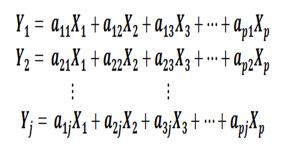
\includegraphics[]{Capture4.JPG}
\centering
\end{figure}

\end{comment}



\begin{comment}
\subsection{Network Time Protocol}

Sinkronisasi waktu jaringan mengacu pada penyimpangan batas waktu yang dilakukan oleh berbagai komunikasi atau komputer perangkat dalam jaringan dalam rentang yang cukup kecil\cite{ntp1}, sinkronisasi waktu pada jaringan dan server dapat dilakukan dengan berbagai metode, salah satunya adalah NTP. Keunggulan dari NTP memiliki akurasi tinggi serta dapat menggunakan berbagai alat sebagai referensi waktu seperti GPS, Time Code d.l.l. NTP bekerja dengan cara klien NTP memulai pertukaran permintaan waktu dengan server NTP. Sebagai hasil dari pertukaran ini, klien dapat menghitung penundaan tautan dan offset lokalnya, dan menyesuaikan jam lokal agar sesuai dengan jam di komputer server.

Dibandingkan dengan protokol lainnya untuk sinkronisasi waktu seperti SNTP (Simple Network Time Protocol), NTP dapat lebih andal karena dapat menerima input waktu dari berbagai sumber sedangkan SNTP hanya dapat menggunakan satu sumber input waktu, dari jam hardware atau jam interface jaringan. Namun, kedua protocol ini dapat bertukar informasi mengenai waktu sehingga lebih memudahkan dalam perancangan sistem.
\end{comment}

%\subsection{Distributed Denial of Service}

\subsection{Dataset}

Dataset yang akan digunakan adalah NSL KDD \texttt{(github.com/defcom17/NSL\_KDD)} karena dataset KDD lama sudah tidak diperbaharui lagi sejak 1999 sehingga sudah tidak relevan dengan gambaran serangn DoS saat ini.
Data yang digunakan sendiri berjumlah 130.440 dengan koneksi bertipe normal sebanyak 77053, dos sebanyak 53387.
Selain itu ada data log, data log adalah data yang diperoleh dari log snort pada server percobaan dan kemudian data dri log tersebut di-generate menjadi dataset baru

\subsection{Server}
\subsubsection{Operating System}

\textit{Operating System} yang akan digunakan adalah Linux OS dengan Ubuntu versi 18.04 karena fleksibilitas dari ubuntu dan dukungan dari komunitas yang banyak membuat ubuntu sesuai untuk dijadikan platform ubntuk percobaan.

\subsubsection{IDS (\textit{Intrusion Detection System})}
Snort adalah \textit{Network Intrusion Detection System} (NIDS) \textit{open source} yang mampu melakukan analisis lalu lintas jaringan secara \textit{real-time} dan paket logging pada jaringan. Snort juga dapat melakukan analisis protokol, pencarian / pencocokan konten, dan dapat digunakan untuk mendeteksi berbagai serangan dan probe, seperti buffer overflows, \textit{stealth port scans}, serangan CGI, probe SMB, percobaan SMB, dan banyak lagi.

\subsection{Desain Sistem}

\begin{figure}[H]
\centering
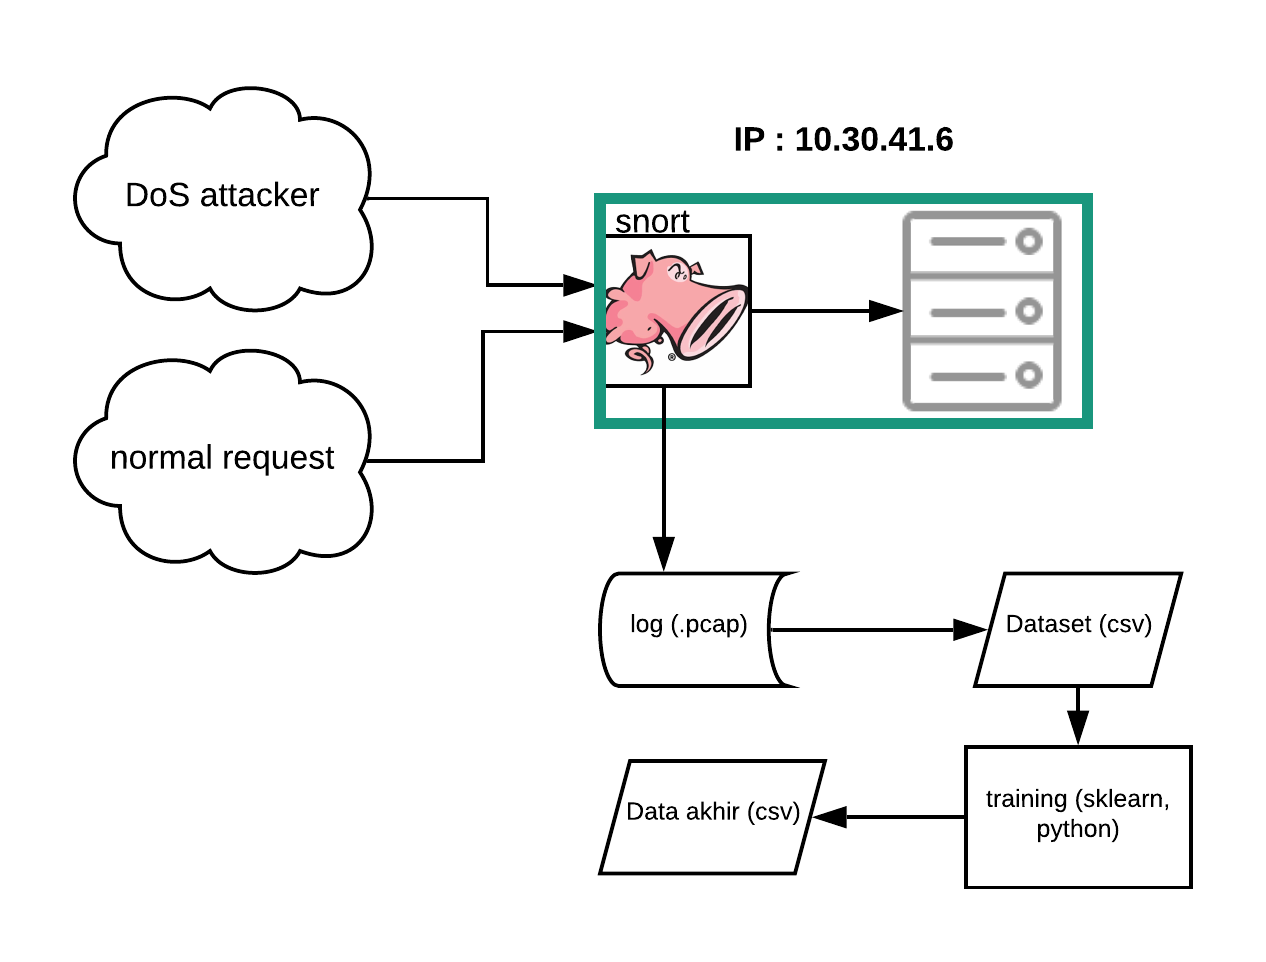
\includegraphics[width=10cm]{tugas akhir.png}
\caption{desain sistem}
\end{figure}

Snort dan server (web) berada pada satu fisik komputer. Serangan berasal dari 1 lokasi yang sama (tergantung pemilihan lokasi pada VPS), normal ping berasal dari region yang sama dengan server.

data log berasal dari snort yang memiliki format .pcap akan digenerate menjadi dataset yang sesuai dengan format NSL KDD.

\begin{itemize}
	\item Normal ping merupakan ping biasa dari sebuah ubuntu \textit{machine}.
	\item Snort Rule digenerate awal berdasarkan karakteristik.
\end{itemize}

\subsection{Tipe koneksi serangan}
\begin{itemize}
    \item TCP Flood
    \item UDP Flood
    \item ICMP Flood
\end{itemize}

Serangan dilakukan menggunakan tiga metode diatas diharapkan menghasilkan data yang komprehensif untuk diuji menggunakan aNN.

%%%%%%%%%%%%%%%%% BAB III %%%%%%%%%%%%%
\section{Pengujian}


\subsection{Percobaan}

\begin{figure}[H]
\centering
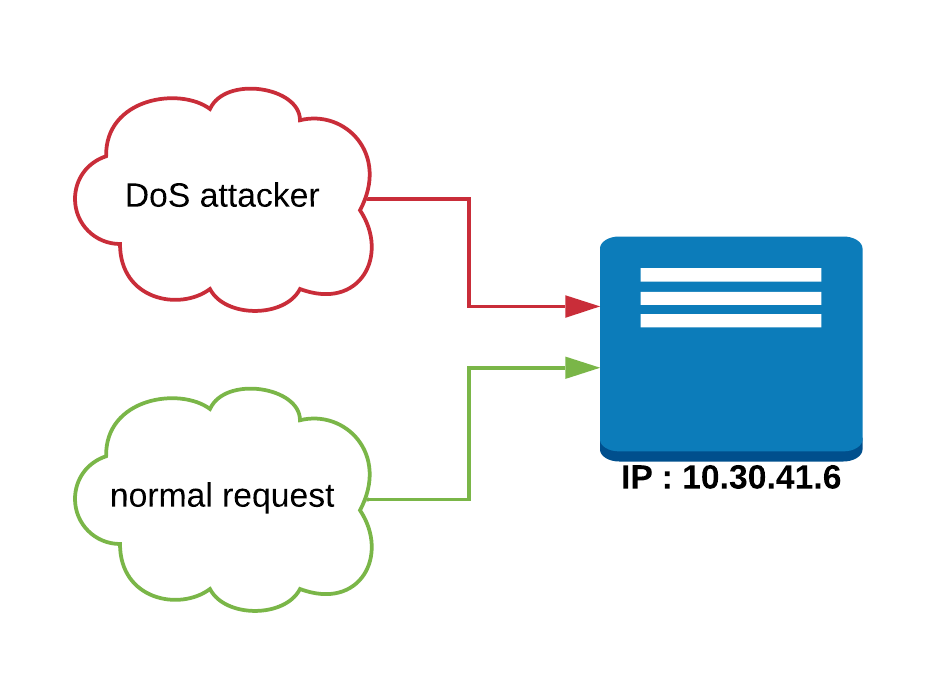
\includegraphics[width=0.5\textwidth]{skenario}
\caption{Visualisasi serangan}
\label{fig:figure2}
\end{figure}

Percobaan dilakukan dengan melakukan dos terhadap \textit{server} dengan disertai ping normal terhadap \textit{server.}

\textit{DoS Attacker} adalah serangan yang dijelaskan pada bab 3.4 sedangkan normal ping adalah \textit{request} normal dari \textit{host} lain selain \textit{attacker}.



\subsection{Snort}
Rules pada snort diterapkan berbeda-beda untuk setiap jenis serangan dengan harapan serangan DDoS yang dilakukan dapat tersaring dengan baik pada rule tersebut.

Contoh rule snort untuk serangan TCP-SYN Flood : 

\begin{lstlisting}
alert tcp !$HOME_NET any -> $HOME_NET 80 (flags: S; msg:"Possible TCP DoS"; 
flow: stateless; threshold: type both, track by_dst)
\end{lstlisting}

\subsection{Hasil Data}
Data yang didapatakan adalah sebanyak 1850 data dari log snort. Data ini terbagi menjadi dua kategori, data normal dan data DoS.

\subsection{Serangan}
\subsubsection{TCP Flood}
Pada serangan berjenis \textit{TCP Flood} ini data yang diperoleh sebanyak 1559. Serangan dengan metode TCP Flooding menggunakan Metasploit dengan TCP SYN Flooder. \\

\textit{Contoh perintah metasploit} :

\begin{lstlisting}
sudo msfconsole 
$ use auxiliary/dos/tcp/synflood 
$ set RHOSTS 10.30.41.6
$ set RPORT 80
$ run or $ exploit
\end{lstlisting}

atau bila menggunakan Hping 3 :

\begin{lstlisting}
$ sudo hping3 --tcp -c 15000 -d 120 -S -w 64 -p 80 --flood --rand-source 10.30.41.6
\end{lstlisting}


\subsubsection{UDP Flood}
Pada serangan berjenis \textit{UDP Flood} ini data yang diperoleh sebanyak 197. Serangan dilakukan dengan menggunakan Hping3. \newline

Perintah yang digunakan :

\begin{lstlisting}
$ sudo hping3 --udp -p 80 --flood --rand-source 10.30.41.6
\end{lstlisting}


\subsubsection{ICMP Flood}
Pada serangan berjenis \textit{ICMP Flood} ini data yang diperoleh sebanyak 94, pada skenario serangan juga dilakukan dengan menggunakan Hping3.

Perintah yang digunakan :
\begin{lstlisting}
$ sudo hping3 --icmp -p 80 --flood --rand-source 10.30.41.6
\end{lstlisting}

\subsection{Pengumpulan Log}
\subsubsection{Log snort}
Log dari snort dikumpulkan melalui server lokal karena percobaan menggunakan server daring selalu mengalami kegagalan dan diblok oleh firewall \textit{provider} dari \textit{Virtual Private Server} (VPS).

\subsubsection{Konversi ke CSV}
Data yang dihasilkan dari log snort berupa file .pcap kemudian dikonversi menjadi \textit{file} .csv, pemilihan \textit{command} pada \textit{tools} hping3 juga memiliki peran dimana \textit{command} ini menentukan beberapa nilai pada fitur dataset yang akan digunakan untuk tes model.

\subsection{Klasifikasi hasil}
Klasifikasi data menggunakan Python 3 dan scikit-learn sebagai library utama, langkah pertama adalah dengan \textit{training} dataset dari NSL KDD dan didapatkan akurasi 99,88\%, kemudian didapatkan model dari \textit{trainig} data ini dan dites ke datalog yang didapatkan dari log snort.

Kemudian dilakukan eliminasi fitur pada dataset NSL KDD berdasarkan \cite{kdd99_feature} dan menghasilkan akurasi 99,40\% dan model dari hasil \textit{training} ini dites ke dataset yang berasal dari log snort yang fitur pada datasetnya telah dielimnasi juga.

\subsubsection{Data Asli}
Akurasi klasifikasi fitur lengkap 99,88\%, akurasi dengan fitur terseleksi berdasarkan \cite{kdd99_feature} adalah 99,40\%.

\subsubsection{Data Berasal dari Log Snort}
Akurasi klasifikasi dengan fitur lengkap 92,84\%, akurasi dengan fitur terseleksi berdasarkan \cite{kdd99_feature} adalah 92,36\%.


%%%%%%%%%%%%%%%%%%%%%%%%%%% BAB IV %%%%%%%%%%%%%%%%%%%%%

\section{Evaluasi}
\subsection{Hasil Serangan}
Hasil serangan menghasilkan datalog yang dapat digunakan untuk membuktikan akurasi algoritma aNN. Serangan dilakukan dengan tiga metode yang telah disebutkan di 3.4, hasil klasifikasi data dapat dilihat pada tabel 2.

\begin{table}[h]
\begin{center}
\begin{tabular}{|c|c|c|c|}
\hline
No & Data      & Jumlah Fitur & Akurasi \\ \hline
1  & Train Tes & 41           & 99.88\% \\ \hline
2  & Data Log  & 41           & 92.60\% \\ \hline
3  & Train Tes & 24           & 99.45\% \\ \hline
4  & Data Log  & 24           & 92.36\% \\ \hline
\end{tabular}
\caption{\label{tab:table-name}Hasil klasifikasi.}
\end{center}
\end{table}

\subsection{Klasifikasi dengan fitur lengkap}
Dengan fitur lengkap untuk melakukan klasifikasi DDoS, akurasi yang didapatkan adalah 99,88\% ketika model dites dengan data dari log akurasi yang didapat adalah 99,60\%

\subsection{Klasifikasi dengan fitur terseleksi}
Dengan fitur lengkap untuk melakukan klasifikasi DDoS, akurasi yang didapatkan adalah 99.45\%, setelah dites dengan data dari log didapatkan akurasi 92,36\%.

\begin{comment}
\subsection{Hardware Usage}
XXXXXXX
\end{comment}

\section{Kesimpulan}

Dengan fitur terseleksi pada dataset membuktikan bahwa data dapat diproses dengan waktu yang lebih cepat meski tanpa \textit{treatment} data yang lebih rumit, namun hasil akurasi klasifikasi mengalami penutusan yang cukup signifikan mencapai 7,52\% dari akurasi klasifikasi yang menggunakan fitur lengkap, dari yang sbelumnya 98,88\% menjadi 92,36\%. 

Penelitian lanjutan dengan metode lain sebaiknya tetap dilakukan terutama menggunakan \textit{hardware} dan library Deep Learning seperti tensorflow untuk hasil akurasi yang lebih baik, selain akurasi yang lebih baik menggunakan Deep Learning, waktu klasifikasi dan \textit{training} menggunakan Deep Learning juga diharapakan lenbih singkat.

\newpage

\bibliographystyle{abbrv}
\bibliography{references}